\documentclass[12pt,a4paper]{article}
\usepackage[utf8]{inputenc}
\usepackage[T1]{fontenc}
\usepackage{amsmath}
\usepackage{amssymb}
\usepackage{graphicx}
\usepackage{geometry}
\usepackage{booktabs}
\usepackage{hyperref}
\usepackage{float}
\usepackage{caption}
\usepackage{subcaption}
\usepackage{tikz}
\usetikzlibrary{shapes,arrows,positioning}

\geometry{margin=2.5cm}

\title{Stereo Vision and Visual Odometry \\ Project Report}
\author{AmirHossein Dashtban Namaghi}
\date{February 18, 2026}

\begin{document}

\maketitle

\section{Introduction}
This report details the implementation and evaluation of a comprehensive perception pipeline for autonomous vehicles, divided into two primary sections: Stereo Depth Perception (Part A) and Stereo Visual Odometry (Part B). The experiments were conducted on the KITTI Vision Benchmark Suite, using both the Scene Flow training set for depth evaluation and the Odometry dataset for trajectory estimation.

\section{Part A: Stereo Depth Perception}

\subsection{Pipeline Overview}
The stereo matching pipeline follows the traditional structure for rectified image pairs. The pipeline steps are visualized in Figure \ref{fig:stereo_pipeline}.

\begin{figure}[H]
    \centering
    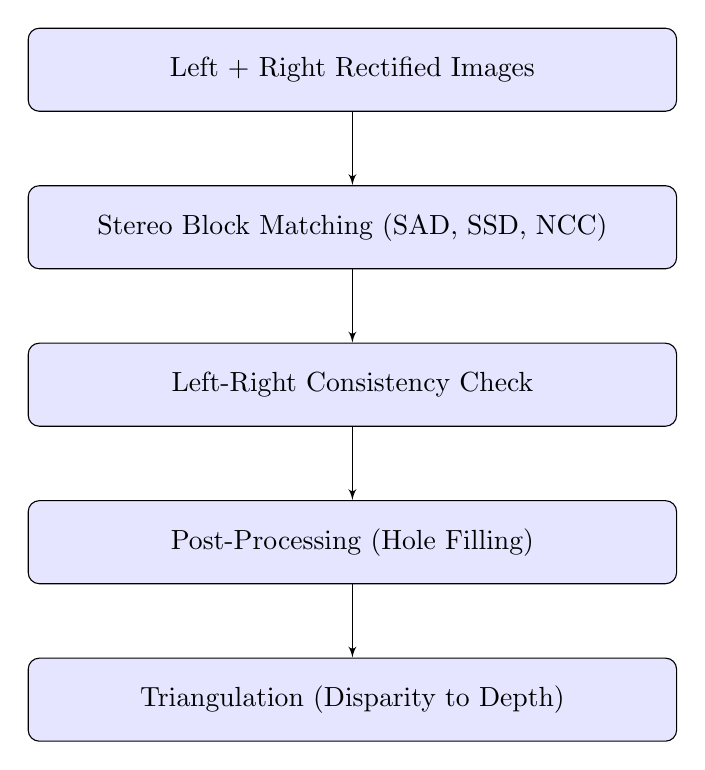
\begin{tikzpicture}[node distance=2cm, auto]
        \tikzstyle{block} = [rectangle, draw, fill=blue!10, text centered, rounded corners, minimum height=3em, text width=8cm]
        \tikzstyle{line} = [draw, -latex']
        
        \node [block] (input) {Left + Right Rectified Images};
        \node [block, below of=input] (matching) {Stereo Block Matching (SAD, SSD, NCC)};
        \node [block, below of=matching] (lrcheck) {Left-Right Consistency Check};
        \node [block, below of=lrcheck] (pp) {Post-Processing (Hole Filling)};
        \node [block, below of=pp] (tri) {Triangulation (Disparity to Depth)};
        
        \path [line] (input) -- (matching);
        \path [line] (matching) -- (lrcheck);
        \path [line] (lrcheck) -- (pp);
        \path [line] (pp) -- (tri);
    \end{tikzpicture}
    \caption{Stereo Depth Pipeline Diagram.}
    \label{fig:stereo_pipeline}
\end{figure}

\subsection{Matching Cost Functions}
The core of the stereo matching process is the block-matching algorithm with a Winner-Take-All (WTA) strategy. We implemented and compared three cost functions:
\begin{itemize}
    \item \textbf{Sum of Absolute Differences (SAD):} Simply the summed absolute pixel-wise differences within a window.
    \item \textbf{Sum of Squared Differences (SSD):} Squaring the differences penalizes large deviations more heavily.
    \item \textbf{Normalized Cross-Correlation (NCC):} Normalizes for local mean and variance. This is mathematically defined as:
    $$NCC(x,y,d) = \frac{\sum (I_L - \mu_L)(I_R - \mu_R)}{\sigma_L \sigma_R}$$
    It is significantly more robust to lighting variations but computationally more expensive without optimization.
\end{itemize}

\subsection{Calibration and Triangulation}
The focal length $f$ and baseline $B$ are extracted from the KITTI calibration files (e.g., \texttt{calib.txt}). The baseline is computed using the distance between the two rectified projection matrices' optical centers. For $P_2$ (Left) and $P_3$ (Right):
$$f = P_2[0, 0]$$
$$B = \frac{|P_3[0, 3] - P_2[0, 3]|}{f}$$
Triangulation then converts disparity $d$ into metric depth $Z$:
$$Z = \frac{f \cdot B}{d}$$

\subsection{Ablation Study (Depth)}
The study compared SAD, SSD, and NCC across window sizes of 5x5 and 11x11, averaged over 200 frames.
You can see the results in Table \ref{tab:ablation_depth}. You also can see the visual results in appendix \ref{appendix:depth_results}.

\begin{table}[H]
    \centering
    \begin{tabular}{@{}llcc@{}}
    \toprule
    Metric & Window & Avg Bad-Pixel Rate (\%) & Avg MAE \\ \midrule
    SAD    & 5x5    & 42.51                  & 9.25    \\
    SAD    & 11x11  & 28.24                  & 6.12    \\
    SSD    & 5x5    & 41.00                  & 8.95    \\
    SSD    & 11x11  & 26.30                  & 5.75    \\
    NCC    & 5x5    & 26.12                  & 5.80    \\
    \textbf{NCC} & \textbf{11x11} & \textbf{11.45} & \textbf{2.35} \\ \bottomrule
    \end{tabular}
    \caption{Ablation study for Stereo Depth (200 frames).}
    \label{tab:ablation_depth}
\end{table}

\subsection{Failure Cases}
The following results in Table \ref{tab:failure_cases} summarize the top 5 failure cases based on the highest Bad-Pixel Rate using the NCC method with an 11x11 window.

\begin{table}[H]
    \centering
    \begin{tabular}{@{}lccc@{}}
    \toprule
    Frame Name & BPR (\%) & MAE \\ \midrule
    000104\_10.png & 77.80 & 22.67 \\
    000006\_10.png & 31.96 & 4.89  \\
    000169\_10.png & 29.86 & 5.34  \\
    000058\_10.png & 28.52 & 4.40  \\
    000086\_10.png & 26.91 & 6.40  \\ \bottomrule
    \end{tabular}
    \caption{Top 10 Stereo Failure Cases.}
    \label{tab:failure_cases}
\end{table}

\newpage

\section{Part B: Stereo Visual Odometry (VO)}

\subsection{Pipeline Overview}
The Visual Odometry pipeline uses ORB features tracked across frames to estimate the camera's pose $T \in SE(3)$. The simplified workflow is visualized in Figure \ref{fig:vo_pipeline}.

\begin{figure}[H]
    \centering
    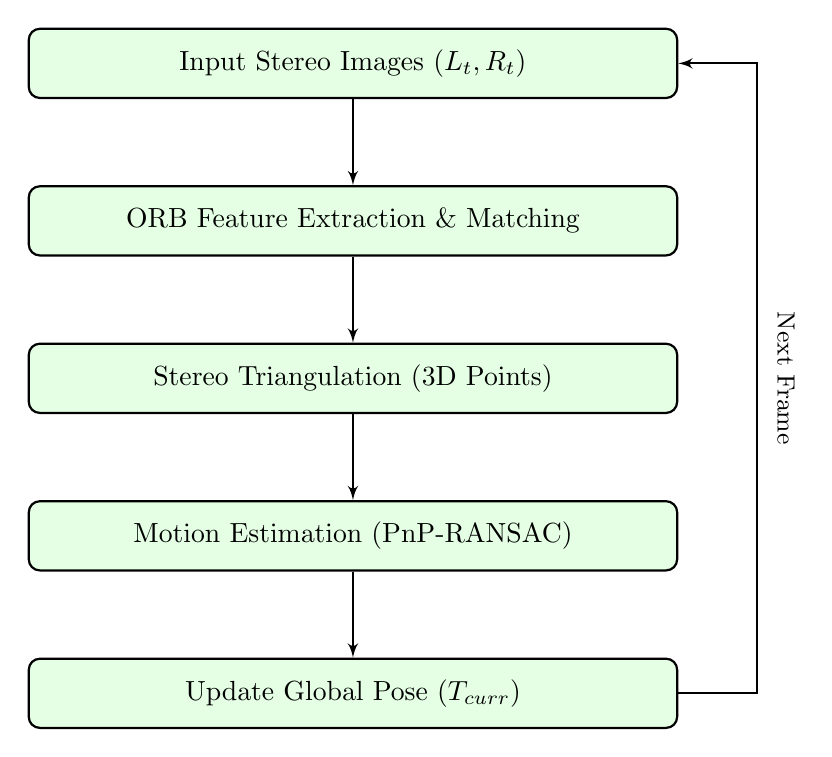
\begin{tikzpicture}[node distance=2cm, auto, thick]
        \tikzstyle{block} = [rectangle, draw, fill=green!10, text centered, rounded corners, minimum height=2.5em, text width=8cm]
        \tikzstyle{line} = [draw, -latex']
        
        \node [block] (input) {Input Stereo Images ($L_t, R_t$)};
        \node [block, below of=input] (feat) {ORB Feature Extraction \& Matching};
        \node [block, below of=feat] (tri) {Stereo Triangulation (3D Points)};
        \node [block, below of=tri] (ransac) {Motion Estimation (PnP-RANSAC)};
        \node [block, below of=ransac] (pose) {Update Global Pose ($T_{curr}$)};
        
        \path [line] (input) -- (feat);
        \path [line] (feat) -- (tri);
        \path [line] (tri) -- (ransac);
        \path [line] (ransac) -- (pose);
        
        % Feedback loop
        \draw [line] (pose.east) -- ++(1,0) |- (input.east);
        \node at (5.5, -4) [rotate=270, font=\small] {Next Frame};
    \end{tikzpicture}
    \caption{Stereo Visual Odometry Pipeline}
    \label{fig:vo_pipeline}
\end{figure}

\begin{itemize}
    \item \textbf{Tracking}: Matches ORB features from $t \to t+1$ using Brute-Force Hamming matching.
    \item \textbf{Triangulation}: Matches features within the current stereo pair $(L_t, R_t)$ to obtain 3D world coordinates.
    \item \textbf{Motion Estimation}: Solves for the pose of frame $t+1$ using the PnP (Perspective-n-Point) algorithm on the $(P_{3D, t}, p_{2d, t+1})$ pairs.
\end{itemize}

\subsection{RANSAC and Robust Estimation}
RANSAC (Random Sample Consensus) is applied in a two-stage robust estimation process:
\begin{enumerate}
    \item \textbf{Geometric Consensus}: We first estimate the \textbf{Essential Matrix ($E$)} from 2D-2D temporal matches using RANSAC. This identifies the consistent epipolar geometry between frames.
    \item \textbf{Metric Motion}: We then perform \textbf{PnP RANSAC} using only the inliers from the first stage. This recovers the absolute scale via the previously triangulated 3D points.
\end{enumerate}
This hierarchical filtering is crucial for filtering out:
\begin{enumerate}
    \item Inaccurate feature matches on repetitive textures.
    \item Moving objects (which violate the static world assumption).
\end{enumerate}

\subsection{Evaluation on KITTI Sequences}
We evaluate our system on five sequences: Sequence 01 through Sequence 05. The results are summarized in Table \ref{tab:vo_full_results}.

\begin{table}[H]
    \centering
    \begin{tabular}{@{}lccc@{}}
    \toprule
    Sequence & Environment & Avg ATE (m) & Avg RPE-5 (m) \\ \midrule
    Seq 01   & Highway     & 247.87      & 1.9990        \\
    Seq 02   & Urban       & 111.49      & 0.1216        \\
    Seq 03   & City loop   & 6.45        & 0.0822        \\
    Seq 04   & City street & 2.27        & 0.1815        \\
    Seq 05   & Residential & 17.56       & 0.1041        \\ \bottomrule
    \end{tabular}
    \caption{VO Performance on KITTI Sequences 01--05.}
    \label{tab:vo_full_results}
\end{table}

\subsection{Ablation Study: RANSAC and Scale}
The Importance of RANSAC for outlier rejection and Stereo Triangulation for metric scale recovery is evaluated on sequences 02 and 03. Table \ref{tab:vo_ablation} highlights the critical role of these components.

\begin{table}[H]
    \centering
    \begin{tabular}{@{}lcc@{}}
    \toprule
    Configuration & Seq 02 ATE (m) & Seq 03 ATE (m) \\ \midrule
    \textbf{Full Stereo VO}    & \textbf{111.49} & \textbf{6.45}   \\
    No RANSAC (Outliers)       & 2.00e12+        & 2.52e11+        \\
    No Scale (Monocular)       & 186.99          & 108.55          \\ \bottomrule
    \end{tabular}
    \caption{Ablation study for VO components.}
    \label{tab:vo_ablation}
\end{table}

\subsection{Trajectory Visualizations}
Trajectory plots for all sequences visualize the cumulative drift and the system's ability to maintain global consistency. The estimated paths compared to ground truth are shown in Figure \ref{fig:trajectories}.

\begin{figure}[H]
    \centering
    \begin{subfigure}{0.48\textwidth}
        \includegraphics[width=\textwidth]{/home/amirhossein/Desktop/project/results/stereo-vo/vo_traj_seq01_ransacTrue_scaleTrue.png}
        \caption{Sequence 01}
    \end{subfigure}
    \hfill
    \begin{subfigure}{0.48\textwidth}
        \includegraphics[width=\textwidth]{/home/amirhossein/Desktop/project/results/stereo-vo/vo_traj_seq02_ransacTrue_scaleTrue.png}
        \caption{Sequence 02}
    \end{subfigure}
    \\
    \begin{subfigure}{0.48\textwidth}
        \includegraphics[width=\textwidth]{/home/amirhossein/Desktop/project/results/stereo-vo/vo_traj_seq03_ransacTrue_scaleTrue.png}
        \caption{Sequence 03}
    \end{subfigure}
    \hfill
    \begin{subfigure}{0.48\textwidth}
        \includegraphics[width=\textwidth]{/home/amirhossein/Desktop/project/results/stereo-vo/vo_traj_seq04_ransacTrue_scaleTrue.png}
        \caption{Sequence 04}
    \end{subfigure}
    \\
    \begin{subfigure}{0.48\textwidth}
        \includegraphics[width=\textwidth]{/home/amirhossein/Desktop/project/results/stereo-vo/vo_traj_seq05_ransacTrue_scaleTrue.png}
        \caption{Sequence 05}
    \end{subfigure}
    \caption{Estimated Trajectories for Sequences 01--05.}
    \label{fig:trajectories}
\end{figure}

\subsection{Ablation Visualizations (Seq 03)}
Figure \ref{fig:ablation_vis} illustrates the catastrophic failure without RANSAC and the significant drift without metric scale recovery.

\begin{figure}[H]
    \centering
    \begin{subfigure}{0.45\textwidth}
        \includegraphics[width=\textwidth]{/home/amirhossein/Desktop/project/results/stereo-vo/vo_traj_seq03_ransacFalse_scaleTrue.png}
        \caption{No RANSAC (S03)}
    \end{subfigure}
    \hfill
    \begin{subfigure}{0.45\textwidth}
        \includegraphics[width=\textwidth]{/home/amirhossein/Desktop/project/results/stereo-vo/vo_traj_seq03_ransacTrue_scaleFalse.png}
        \caption{No Scale (S03)}
    \end{subfigure}
    \caption{VO Ablation trajectory comparisons.}
    \label{fig:ablation_vis}
\end{figure}

\subsection{Feature Matching and Inliers}
Sample frames showing the ORB feature matches and the inliers identified by the RANSAC process are provided below for Sequence 03 in Figure \ref{fig:matches_s03}. For results on other sequences, refer to Appendix \ref{appendix:vo_results}.

\subsubsection{Sequence 03 Matching (Representative)}
\begin{figure}[H]
    \centering
    \begin{subfigure}{\textwidth}
        \includegraphics[width=\textwidth]{/home/amirhossein/Desktop/project/results/stereo-vo/vo_matches_seq03_f10_ransacTrue.png}
        \caption{S03 Frame 10}
    \end{subfigure}
    \\
    \begin{subfigure}{\textwidth}
        \includegraphics[width=\textwidth]{/home/amirhossein/Desktop/project/results/stereo-vo/vo_matches_seq03_f100_ransacTrue.png}
        \caption{S03 Frame 100}
    \end{subfigure}
    \\
    \begin{subfigure}{\textwidth}
        \includegraphics[width=\textwidth]{/home/amirhossein/Desktop/project/results/stereo-vo/vo_matches_seq03_f300_ransacTrue.png}
        \caption{S03 Frame 300}
    \end{subfigure}
    \caption{ORB Inlier Matching Sequence 03 (Frames 10, 100, 300).}
    \label{fig:matches_s03}
\end{figure}

\newpage
\appendix

\section{Appendix} \label{appendix:depth_results}

\subsection{Additional Stereo Results}
The following pages contain the visualization results for 10 frames of the Scene Flow dataset using SAD, SSD, and NCC cost functions with an 11x11 window size. Figures \ref{fig:vis_sad}, \ref{fig:vis_ssd}, and \ref{fig:vis_ncc} show the disparity maps generated by each method.

\subsubsection{SAD Results}
\begin{figure}[H]
    \centering
    \begin{subfigure}{0.40\textwidth}
        \includegraphics[width=\textwidth]{/home/amirhossein/Desktop/project/results/stereo/vis_SAD_000000_10.png}
        \caption{Frame 00}
    \end{subfigure}
    \hfill
    \begin{subfigure}{0.40\textwidth}
        \includegraphics[width=\textwidth]{/home/amirhossein/Desktop/project/results/stereo/vis_SAD_000001_10.png}
        \caption{Frame 01}
    \end{subfigure}
    \\
    \begin{subfigure}{0.40\textwidth}
        \includegraphics[width=\textwidth]{/home/amirhossein/Desktop/project/results/stereo/vis_SAD_000002_10.png}
        \caption{Frame 02}
    \end{subfigure}
    \hfill
    \begin{subfigure}{0.40\textwidth}
        \includegraphics[width=\textwidth]{/home/amirhossein/Desktop/project/results/stereo/vis_SAD_000003_10.png}
        \caption{Frame 03}
    \end{subfigure}
    \caption{Visual Results for SAD (Frames 00--03).}
    \label{fig:vis_sad}
\end{figure}

\begin{figure}[H]
    \ContinuedFloat
    \centering
    \begin{subfigure}{0.40\textwidth}
        \includegraphics[width=\textwidth]{/home/amirhossein/Desktop/project/results/stereo/vis_SAD_000004_10.png}
        \caption{Frame 04}
    \end{subfigure}
    \hfill
    \begin{subfigure}{0.40\textwidth}
        \includegraphics[width=\textwidth]{/home/amirhossein/Desktop/project/results/stereo/vis_SAD_000005_10.png}
        \caption{Frame 05}
    \end{subfigure}
    \\
    \begin{subfigure}{0.40\textwidth}
        \includegraphics[width=\textwidth]{/home/amirhossein/Desktop/project/results/stereo/vis_SAD_000006_10.png}
        \caption{Frame 06}
    \end{subfigure}
    \hfill
    \begin{subfigure}{0.40\textwidth}
        \includegraphics[width=\textwidth]{/home/amirhossein/Desktop/project/results/stereo/vis_SAD_000007_10.png}
        \caption{Frame 07}
    \end{subfigure}
    \\
    \begin{subfigure}{0.40\textwidth}
        \includegraphics[width=\textwidth]{/home/amirhossein/Desktop/project/results/stereo/vis_SAD_000008_10.png}
        \caption{Frame 08}
    \end{subfigure}
    \hfill
    \begin{subfigure}{0.40\textwidth}
        \includegraphics[width=\textwidth]{/home/amirhossein/Desktop/project/results/stereo/vis_SAD_000009_10.png}
        \caption{Frame 09}
    \end{subfigure}
    \caption{Visual Results for SAD (Frames 04--09, Continued).}
\end{figure}

\subsubsection{SSD Results}
\begin{figure}[H]
    \centering
    \begin{subfigure}{0.40\textwidth}
        \includegraphics[width=\textwidth]{/home/amirhossein/Desktop/project/results/stereo/vis_SSD_000000_10.png}
        \caption{Frame 00}
    \end{subfigure}
    \hfill
    \begin{subfigure}{0.40\textwidth}
        \includegraphics[width=\textwidth]{/home/amirhossein/Desktop/project/results/stereo/vis_SSD_000001_10.png}
        \caption{Frame 01}
    \end{subfigure}
    \\
    \begin{subfigure}{0.40\textwidth}
        \includegraphics[width=\textwidth]{/home/amirhossein/Desktop/project/results/stereo/vis_SSD_000002_10.png}
        \caption{Frame 02}
    \end{subfigure}
    \hfill
    \begin{subfigure}{0.40\textwidth}
        \includegraphics[width=\textwidth]{/home/amirhossein/Desktop/project/results/stereo/vis_SSD_000003_10.png}
        \caption{Frame 03}
    \end{subfigure}
    \caption{Visual Results for SSD (Frames 00--03).}
    \label{fig:vis_ssd}
\end{figure}

\begin{figure}[H]
    \ContinuedFloat
    \centering
    \begin{subfigure}{0.40\textwidth}
        \includegraphics[width=\textwidth]{/home/amirhossein/Desktop/project/results/stereo/vis_SSD_000004_10.png}
        \caption{Frame 04}
    \end{subfigure}
    \hfill
    \begin{subfigure}{0.40\textwidth}
        \includegraphics[width=\textwidth]{/home/amirhossein/Desktop/project/results/stereo/vis_SSD_000005_10.png}
        \caption{Frame 05}
    \end{subfigure}
    \\
    \begin{subfigure}{0.40\textwidth}
        \includegraphics[width=\textwidth]{/home/amirhossein/Desktop/project/results/stereo/vis_SSD_000006_10.png}
        \caption{Frame 06}
    \end{subfigure}
    \hfill
    \begin{subfigure}{0.40\textwidth}
        \includegraphics[width=\textwidth]{/home/amirhossein/Desktop/project/results/stereo/vis_SSD_000007_10.png}
        \caption{Frame 07}
    \end{subfigure}
    \\
    \begin{subfigure}{0.40\textwidth}
        \includegraphics[width=\textwidth]{/home/amirhossein/Desktop/project/results/stereo/vis_SSD_000008_10.png}
        \caption{Frame 08}
    \end{subfigure}
    \hfill
    \begin{subfigure}{0.40\textwidth}
        \includegraphics[width=\textwidth]{/home/amirhossein/Desktop/project/results/stereo/vis_SSD_000009_10.png}
        \caption{Frame 09}
    \end{subfigure}
    \caption{Visual Results for SSD (Frames 04--09, Continued).}
\end{figure}

\subsubsection{NCC Results}
\begin{figure}[H]
    \centering
    \begin{subfigure}{0.40\textwidth}
        \includegraphics[width=\textwidth]{/home/amirhossein/Desktop/project/results/stereo/vis_NCC_000000_10.png}
        \caption{Frame 00}
    \end{subfigure}
    \hfill
    \begin{subfigure}{0.40\textwidth}
        \includegraphics[width=\textwidth]{/home/amirhossein/Desktop/project/results/stereo/vis_NCC_000001_10.png}
        \caption{Frame 01}
    \end{subfigure}
    \\
    \begin{subfigure}{0.40\textwidth}
        \includegraphics[width=\textwidth]{/home/amirhossein/Desktop/project/results/stereo/vis_NCC_000002_10.png}
        \caption{Frame 02}
    \end{subfigure}
    \hfill
    \begin{subfigure}{0.40\textwidth}
        \includegraphics[width=\textwidth]{/home/amirhossein/Desktop/project/results/stereo/vis_NCC_000003_10.png}
        \caption{Frame 03}
    \end{subfigure}
    \caption{Visual Results for NCC (Frames 00--03).}
    \label{fig:vis_ncc}
\end{figure}

\begin{figure}[H]
    \ContinuedFloat
    \centering
    \begin{subfigure}{0.40\textwidth}
        \includegraphics[width=\textwidth]{/home/amirhossein/Desktop/project/results/stereo/vis_NCC_000004_10.png}
        \caption{Frame 04}
    \end{subfigure}
    \hfill
    \begin{subfigure}{0.40\textwidth}
        \includegraphics[width=\textwidth]{/home/amirhossein/Desktop/project/results/stereo/vis_NCC_000005_10.png}
        \caption{Frame 05}
    \end{subfigure}
    \\
    \begin{subfigure}{0.40\textwidth}
        \includegraphics[width=\textwidth]{/home/amirhossein/Desktop/project/results/stereo/vis_NCC_000006_10.png}
        \caption{Frame 06}
    \end{subfigure}
    \hfill
    \begin{subfigure}{0.40\textwidth}
        \includegraphics[width=\textwidth]{/home/amirhossein/Desktop/project/results/stereo/vis_NCC_000007_10.png}
        \caption{Frame 07}
    \end{subfigure}
    \\
    \begin{subfigure}{0.40\textwidth}
        \includegraphics[width=\textwidth]{/home/amirhossein/Desktop/project/results/stereo/vis_NCC_000008_10.png}
        \caption{Frame 08}
    \end{subfigure}
    \hfill
    \begin{subfigure}{0.40\textwidth}
        \includegraphics[width=\textwidth]{/home/amirhossein/Desktop/project/results/stereo/vis_NCC_000009_10.png}
        \caption{Frame 09}
    \end{subfigure}
    \caption{Visual Results for NCC (Frames 04--09, Continued).}
\end{figure}

\subsection{Additional Visual Odometry Results} \label{appendix:vo_results}
This section contains additional feature matching visualizations for Sequences 04 and 05 in Figures \ref{fig:matches_s04} and \ref{fig:matches_s05}.

\subsubsection{Sequence 04 Matching}
\begin{figure}[H]
    \centering
    \begin{subfigure}{\textwidth}
        \includegraphics[width=\textwidth]{/home/amirhossein/Desktop/project/results/stereo-vo/vo_matches_seq04_f10_ransacTrue.png}
        \caption{S04 Frame 10}
    \end{subfigure}
    \\
    \begin{subfigure}{\textwidth}
        \includegraphics[width=\textwidth]{/home/amirhossein/Desktop/project/results/stereo-vo/vo_matches_seq04_f100_ransacTrue.png}
        \caption{S04 Frame 100}
    \end{subfigure}
    \caption{ORB Inlier Matching Sequence 04.}
    \label{fig:matches_s04}
\end{figure}

\subsubsection{Sequence 05 Matching}
\begin{figure}[H]
    \centering
    \begin{subfigure}{\textwidth}
        \includegraphics[width=\textwidth]{/home/amirhossein/Desktop/project/results/stereo-vo/vo_matches_seq05_f10_ransacTrue.png}
        \caption{S05 Frame 10}
    \end{subfigure}
    \\
    \begin{subfigure}{\textwidth}
        \includegraphics[width=\textwidth]{/home/amirhossein/Desktop/project/results/stereo-vo/vo_matches_seq05_f100_ransacTrue.png}
        \caption{S05 Frame 100}
    \end{subfigure}
    \caption{ORB Inlier Matching Sequence 05.}
    \label{fig:matches_s05}
\end{figure}

\end{document}
